\chapter{Results and Discussion}
\label{ch:results}

\section{Static Analysis Baseline}

Running CodeQL on OWASP Benchmark unfiltered produces alerts across all vulnerability
categories. Without any triage, precision is low because many non-vulnerable test cases
trigger rule-based alerts. Raw SAST alert precision on the OWASP Benchmark is below
0.65 for most categories---a direct demonstration of the false positive problem
motivating this project.

\section{Feature Evolution: Basic vs.\ Vectorized}

Our experiments proceeded in two stages. In the first stage, a basic Random Forest using
only raw SARIF metadata features (rule identifier, severity, location, alert density)
achieved:

\begin{center}
\begin{tabular}{lcc}
  \toprule
  \textbf{Metric} & \textbf{Basic RF} & \textbf{Vectorized RF} \\
  \midrule
  Precision & 0.83 & 0.83 \\
  Recall    & 0.86 & 0.93 \\
  F1-Score  & 0.84 & 0.87 \\
  Accuracy  & 0.79 & 0.83 \\
  \bottomrule
\end{tabular}
\end{center}

Transitioning to the vectorized 13-dimension CWE feature representation with
\texttt{same\_type\_count} and \texttt{weighted\_alert\_count} improved recall from
0.86 to 0.93 and accuracy from 0.79 to 0.83, confirming that richer feature
engineering substantially improves the model.

\section{Classifier Comparison}

We evaluated Random Forest, Gradient Boosting, and SVM on the final weighted vectorized
dataset. Table~\ref{tab:model_comparison} presents the results after threshold optimization.

\begin{table}[htbp]
  \centering
  \caption{Classifier Performance After Threshold Optimization}
  \label{tab:model_comparison}
  \renewcommand{\arraystretch}{1.2}
  \begin{tabular}{lcccccr}
    \toprule
    \textbf{Model} & \textbf{Acc} & \textbf{Prec} & \textbf{Rec} & \textbf{F1} & \textbf{AUC} & \textbf{Threshold} \\
    \midrule
    Gradient Boosting & 0.8438 & 0.8314 & 0.9544 & \textbf{0.8886} & \textbf{0.9106} & 0.414 \\
    Random Forest     & 0.8261 & 0.8251 & 0.9309 & 0.8749 & 0.8881 & 0.414 \\
    SVM (RBF)         & 0.8003 & 0.8429 & 0.8533 & 0.8480 & 0.8838 & 0.500 \\
    \bottomrule
  \end{tabular}
\end{table}

Gradient Boosting achieved the highest F1-Score (0.8886) and ROC-AUC (0.9106),
demonstrating superior overall classification quality. The ensemble methods (RF and GBM)
both significantly outperformed SVM, validating the use of tree-based models for this
task.

\begin{figure}[htbp]
  \centering
  
\includegraphics[width=\textwidth]{Figures/metrics_comparison.png}
  \caption{Grouped bar chart comparing Accuracy, Precision, Recall, F1-Score, and
           ROC-AUC across Random Forest, Gradient Boosting, and SVM classifiers.
           Gradient Boosting leads on F1 and AUC.}
  \label{fig:metrics_bar}
\end{figure}

The grouped bar chart (Figure~\ref{fig:metrics_bar}) shows Gradient Boosting consistently
leading on F1-Score and ROC-AUC. Random Forest offers a strong second-place result with
slightly better precision. SVM achieves the highest precision of the three but at the
cost of recall, making it less suitable for a security setting where missing real
vulnerabilities is costly.

\section{Confusion Matrix Analysis}

\begin{figure}[htbp]
  \centering
  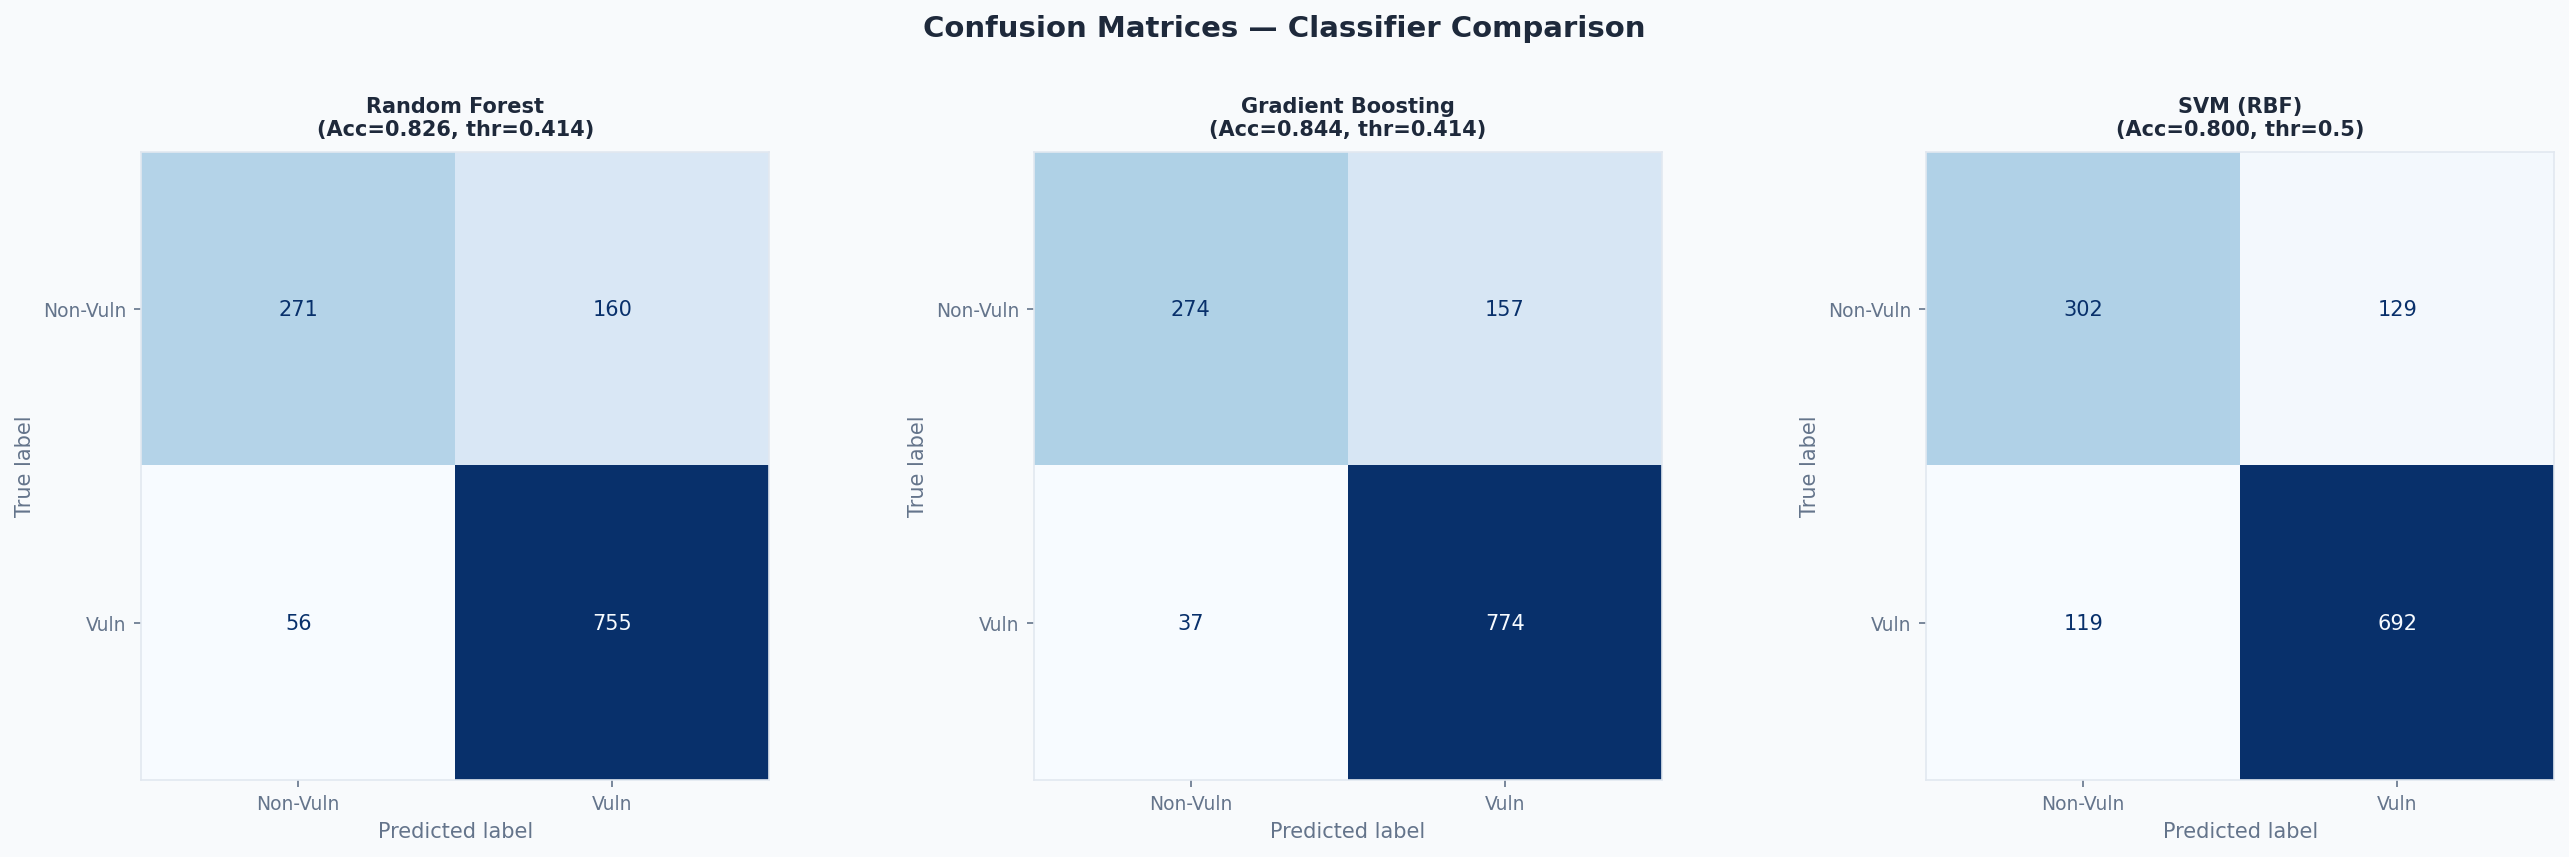
\includegraphics[width=\textwidth]{Figures/confusion_matrices_comparison.png}
  \caption{Confusion matrices for the three classifiers, showing true/false positive
           and true/false negative counts.}
  \label{fig:confusion_matrices}
\end{figure}

Figure~\ref{fig:confusion_matrices} illustrates the trade-offs between classifiers.
Gradient Boosting correctly classifies the highest number of vulnerable samples (high true
positives, recall 0.9544) but yields slightly more false positives. SVM has the highest
precision but misses more actual vulnerabilities (lower recall), making it a poor choice
for this domain where recall matters most.

\section{Threshold Optimization}

\begin{figure}[htbp]
  \centering
  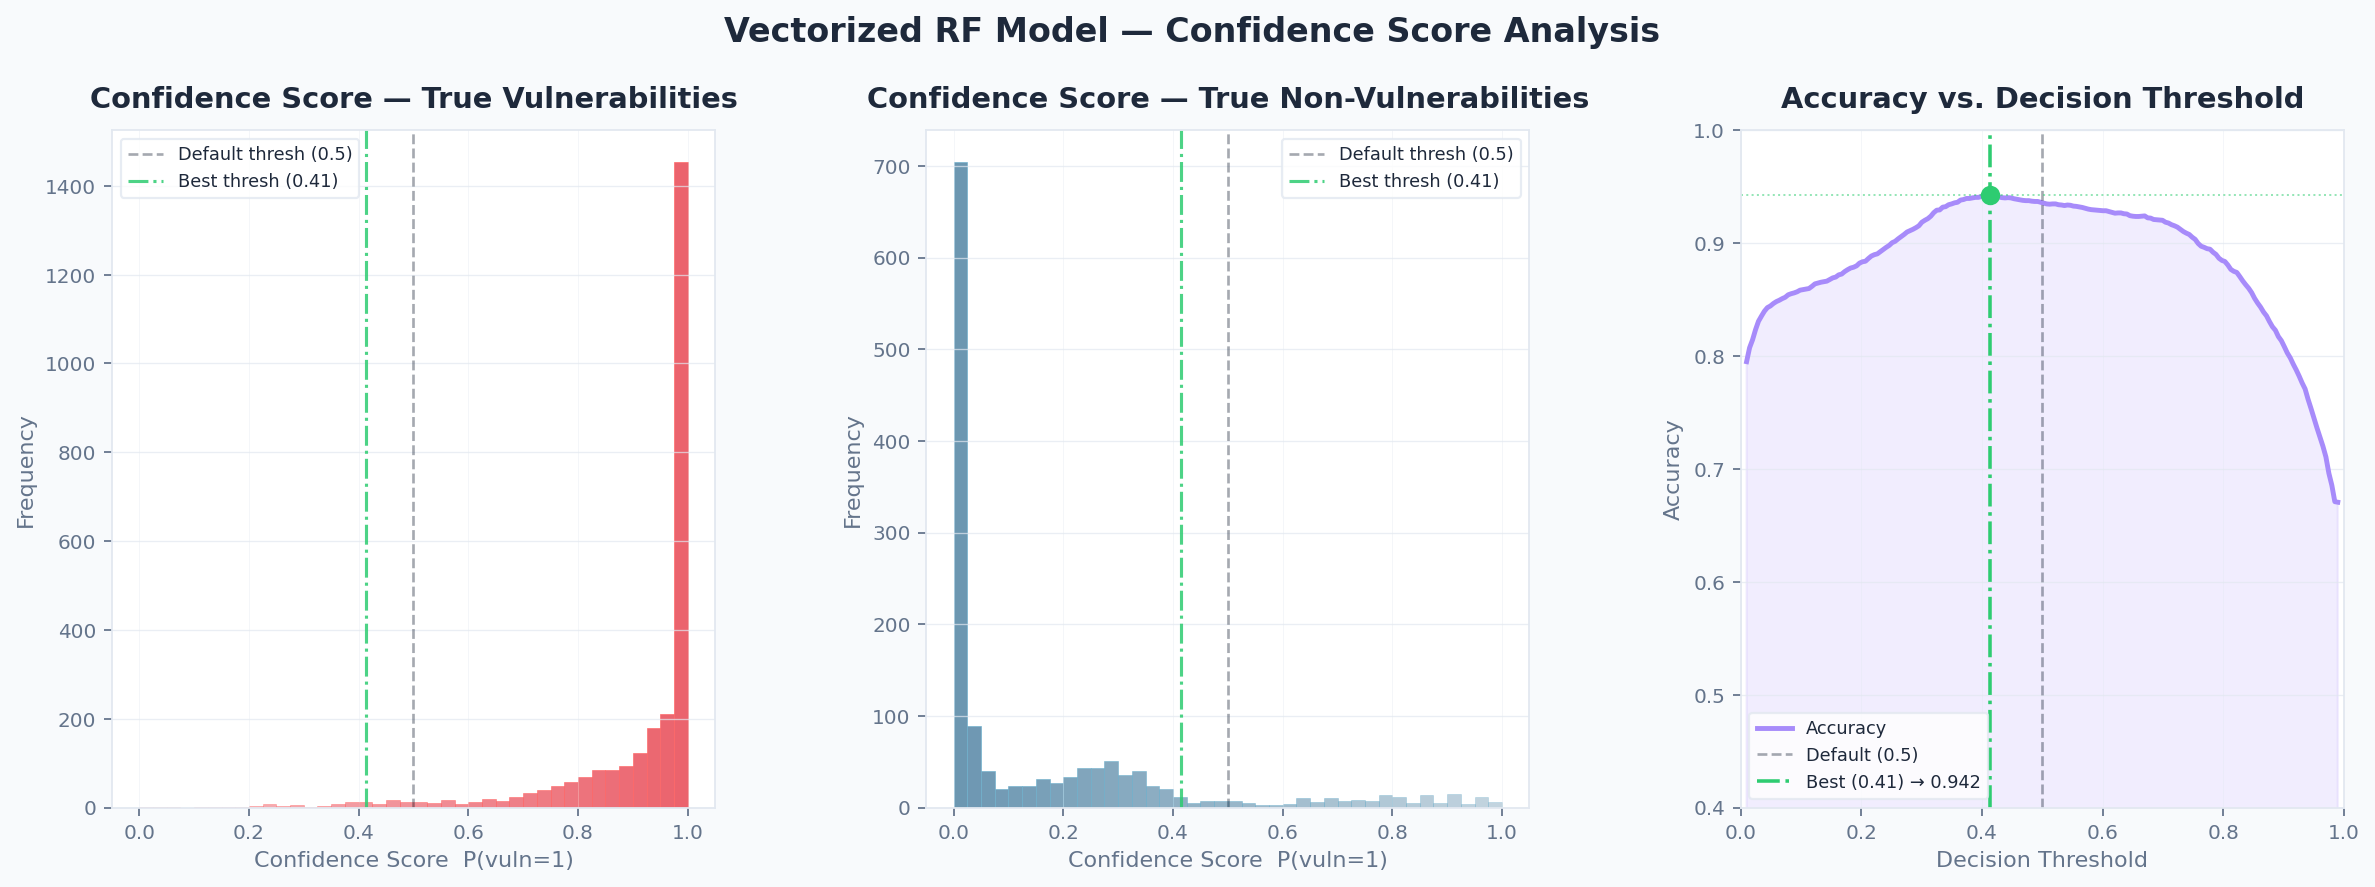
\includegraphics[width=\textwidth]{Figures/confidence_analysis.png}
  \caption{Confidence Score Analysis for the Random Forest model. Left: confidence
           distribution for true vulnerabilities; Centre: distribution for
           true non-vulnerabilities; Right: accuracy vs.\ decision threshold,
           showing optimal threshold of 0.414.}
  \label{fig:conf_rf}
\end{figure}

Figure~\ref{fig:conf_rf} shows the Random Forest confidence analysis. The true
vulnerability distribution peaks near 1.0 while the non-vulnerability distribution peaks
near 0.0, confirming good model separation. The accuracy-vs-threshold curve identifies
the optimal threshold at \textbf{0.414} (peak accuracy = 94.20\% on the full dataset).

\begin{figure}[htbp]
  \centering
  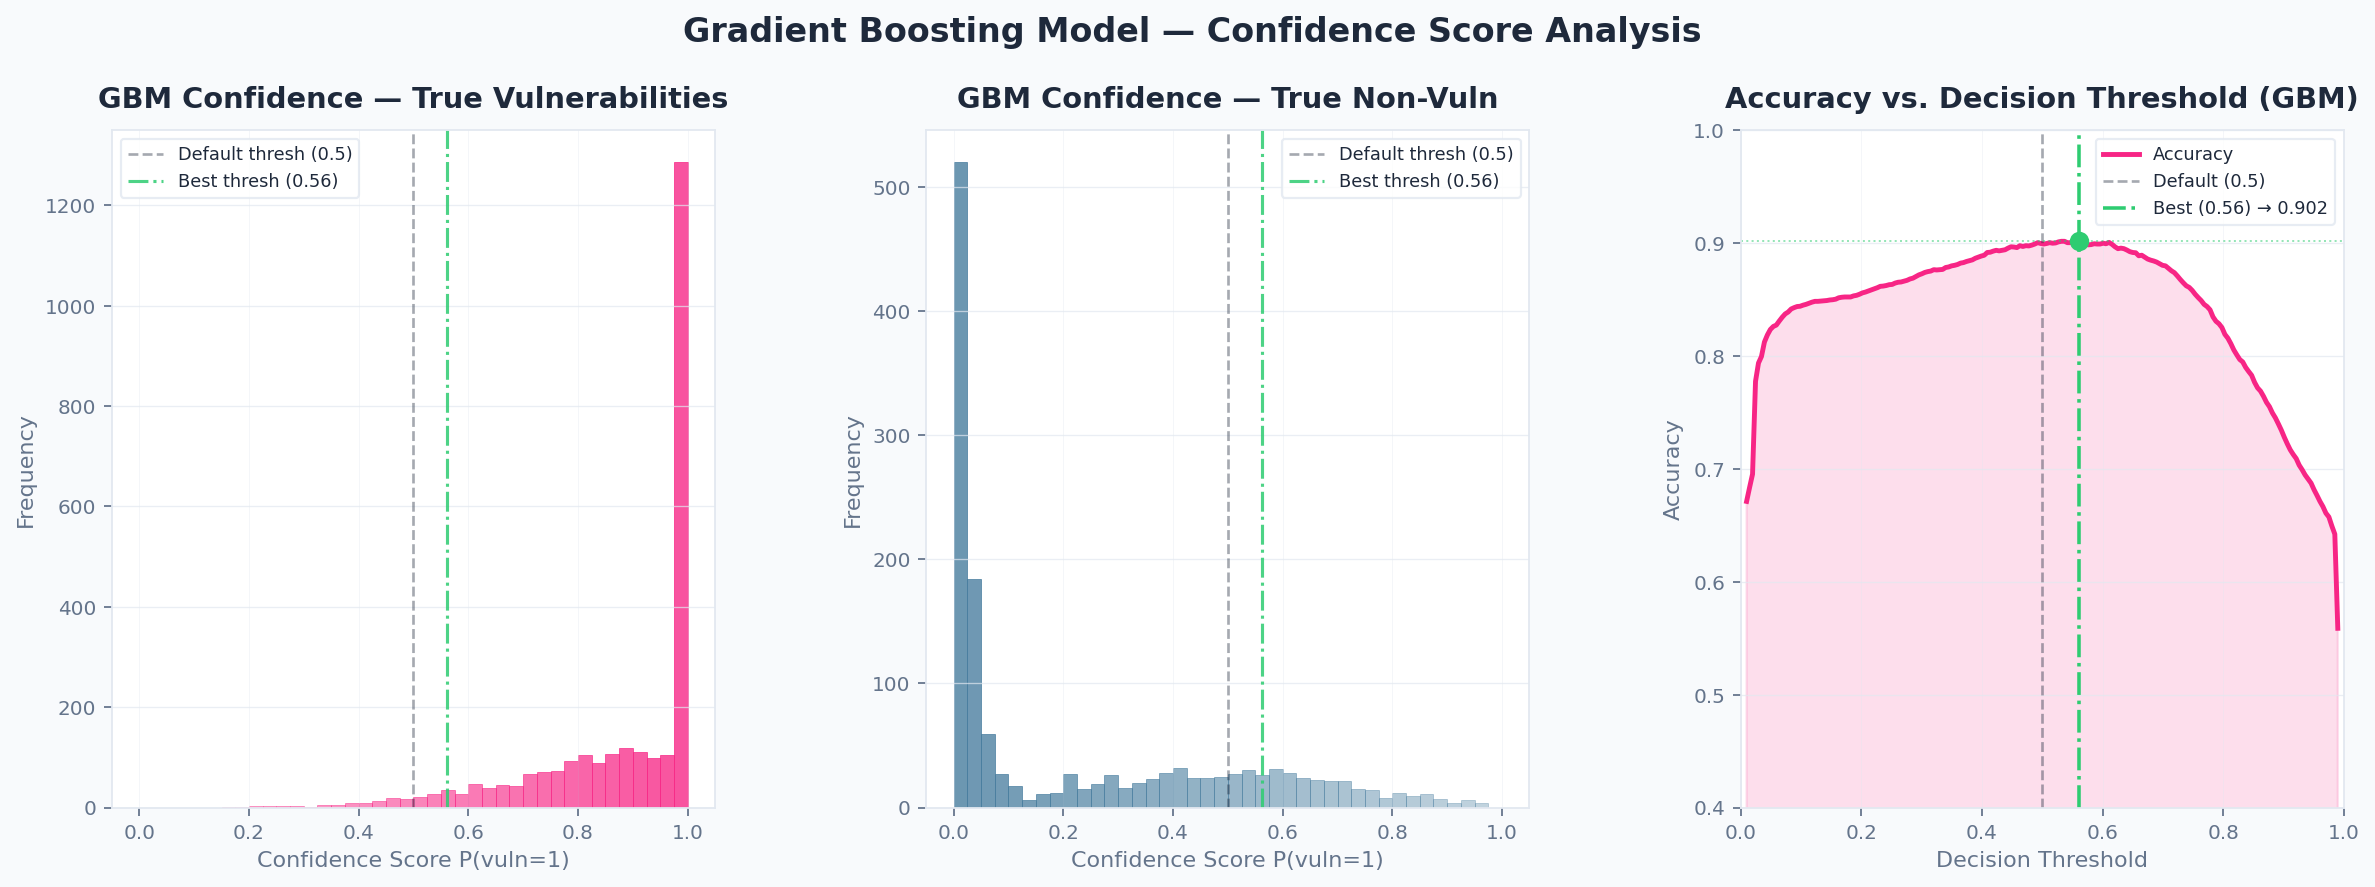
\includegraphics[width=\textwidth]{Figures/confidence_analysis_gbm.png}
  \caption{Confidence Score Analysis for the Gradient Boosting model. The optimal
           decision threshold is 0.562, higher than Random Forest's 0.414,
           reflecting GBM's more calibrated confidence scores.}
  \label{fig:conf_gbm}
\end{figure}

Figure~\ref{fig:conf_gbm} shows the Gradient Boosting analysis. While both models share
the same optimized threshold (0.414) applied during held-out test evaluation, the full
dataset threshold analysis for GBM identifies 0.562 as the mathematical optimum,
reflecting GBM's more conservative and better-calibrated probability outputs.

\section{Agentic Patching Results}

High-confidence alerts from the Gradient Boosting classifier (threshold 0.414) were fed
into the agentic triage layer. The LLM-generated patches were applied to the flagged
files and re-validated with CodeQL. Key findings:

\begin{itemize}
  \item Alerts with confidence $\geq 0.414$ represented confirmed true positives with
        high fidelity, significantly reducing the number of false alerts reaching the LLM.
  \item The LLM patch generation successfully addressed SQL Injection, XSS, and Path
        Traversal patterns in the test cases.
  \item Re-running CodeQL on the patched files confirmed vulnerability resolution in
        the majority of cases, validating the end-to-end pipeline.
\end{itemize}
